\newcommand\w[1]{\includegraphics[width=0.3\textwidth]{#1}}

\section{Representation}

\subsection{Diagrams}
\begin{frame}{\secname: \subsecname}
Fingers are named $L1,\cdots, L5$ and $R1,\cdots,R5$ from thumb to pinky

\begin{itemize}
    \item \pause Ordered from nearest to furthest
    \pause \begin{center}
    $L1\lt L2\lt L3\lt L4\lt L5$\\
    $R1\lt R2\lt R3\lt R4\lt R5$    
    \end{center}
\end{itemize}

\pause String segments are named by finger $F\in\{L1,\cdots, L5,R1,\cdots,R5\}$
\begin{itemize}[<+(1)->]
    \item $Fn$ is the near string, $Ff$ is the far string
    \item $Lp$ and $Rp$ are palmar strings
\end{itemize}

\pause
\begin{figure}\centering
\def\svgwidth{0.5\columnwidth}
\input{figures/open.pdf_tex}
\end{figure}

\note<6>[item]{ (palmar) when we have a string between $L1$ and $L5$, we give a special name, called palmar string}
\note<7->[item]{ the diagrams are intuitive and very visual, but they are less computer friendly}
\note<7->[item]{ what do computers like? they like array of symbols}

\end{frame}


\subsection{Linear Sequences}
\begin{frame}{\secname: \subsecname}
Two key components
\begin{itemize}[<+(1)->]
    \item Fingers that hold the string
    \item Crossings (with parity)
\end{itemize}

\pause Diagram $\to$ linear sequence

\begin{itemize}[<+(1)->]
    \item Start with left nearest finger and travel clockwise
    \item Visit fingers and crossings (with parity)
\end{itemize}

\pause
\def\svgwidth{0.6\columnwidth}
$$\begin{tikzpicture}
    \node at(0,0){\input{figures/open.pdf_tex}};
    \node[shift={(120pt,0)}] at(0,0){$\mapsto$};
    \node[shift={(170pt,0)}] at(0,0){$L1:L5:R2$};
\end{tikzpicture}$$
\note<5>[item]{travel along the string clockwise}
\note<6>[item]{note down the fingers and crossings with parity}
\end{frame}


\begin{frame}{Linear Sequences with Crossings}
Diagram $\to$ linear sequence
\begin{itemize}[<+(1)->]
    \item Name each crossing as $x_i$ for some $i$
    \item Visit overcrossing $\implies$ write $x_i(o)$
    \item Visit undercrossing $\implies$ write $x_i(u)$
\end{itemize}

\pause
$$\begin{tikzpicture}
    % \node at(0,0){\def\svgwidth{0.6\columnwidth}\input{figures/star.pdf_tex}};
    \node at(0,0){\def\svgwidth{0.6\columnwidth}\input{figures/starc.pdf_tex}};
\end{tikzpicture}$$

$$
\scriptstyle
L1:x_1(o):x_2(o):R5:x_3(o):x_4(o):R1:x_5(o):x_1(u):L5:x_2(u):x_3(u):R2:x_4(u):x_5(u)
$$


\end{frame}
\note[itemize]{
\item if we have $n$ fingers holding the string figure that has $m$ crossings, the sequence will have $n+2m$ symbols
\item in most string figures, having a lot of crossings is what makes them beautiful, and it would be tedious to write down the entire sequence by hand
\item (you see that i cant even fit the linear sequence of this simple star with normal size font)
\item so this gives us more motivation to develop a systematic way of computing the movements so we can let computer do the calculuation
\item the most common movements involve a finger and sometimes a near/far string segment of some other finger, but the problem arises in identifying these segments from the sequence
}


\subsection{Identifying String Segments }

\begin{frame}{\subsecname from Linear Sequences}
\begin{adjustwidth}{-1.5em}{-1.5em}
Consider a subsequence $\ldots:L_i:\ldots$ for any $L_i\in\{L1,\ldots,L5\}$

\begin{itemize}[<+(1)->]
    \item Traverse clockwise \raisebox{-0.45\height}{\includegraphics[width=0.2\textwidth]{figures/leftcw.png}} \pause $\implies \ldots:[L_in] L_i [L_if]:\ldots$
    \item Traverse counterclockwise \raisebox{-0.45\height}{\includegraphics[width=0.2\textwidth]{figures/leftccw.png}} \pause $\implies\ldots: [L_if] L_i [L_in]:\ldots$
\end{itemize}

\pause Similarly for finger $R_i$ on the right hand

\begin{itemize}
    \item \raisebox{-0.45\height}{\includegraphics[width=0.2\textwidth]{figures/rightcw.png}} $\implies \ldots:[R_if]R_i[R_in]:\ldots$
    \item\raisebox{-0.45\height}{\includegraphics[width=0.2\textwidth]{figures/rightccw.png}} $\implies\ldots:[R_in]R_i[R_if]:\ldots$
\end{itemize}
\end{adjustwidth}
\end{frame}

\begin{frame}{\subsecname: Opposite Hand}
\begin{adjustwidth}{-1.5em}{-1.5em}
Consider $\ldots:L2:\ldots:R2:\ldots$

\begin{itemize}[<+(1)->]
    \item Even number of crossings between $L2$ and $R2\implies$ rotation persists\\
    \begin{center}
    \includegraphics[width=0.5\columnwidth]{figures/diff-even.png}
    $$
    [L2n]L2[L2f]:[R2f]R2[R2n]
    $$
    \end{center}
    \item Odd number of crossings between $L2$ and $R2\implies$ rotation reverses\\
    \begin{center}
    \includegraphics[width=0.5\columnwidth]{figures/diff-odd.png}
    $$
    [L2n]L2[L2f]:x_1(u):[R2n]R2[R2f]:x_1(o)
    $$
    \end{center}
\end{itemize}    
\end{adjustwidth}
\end{frame}

\begin{frame}{\subsecname: Same Hand}
\begin{adjustwidth}{-1.5em}{-1.5em}
Consider $\ldots:L2:\ldots:L5:\ldots$

\vfill
\pause
\begin{minipage}{0.5\textwidth}
\begin{center}
Even $\implies$ rotation persists\\
\includegraphics[width=0.3\linewidth]{figures/same-even.png}
\end{center}
$$
\scriptstyle
\ldots:[L2n]L2[L2f]:[L2n]L2[L2f]:\ldots
$$
\end{minipage}
\hfill
\pause
\begin{minipage}{0.5\textwidth}
\begin{center}
Odd $\implies$ rotation reverses\\
\includegraphics[width=0.3\linewidth]{figures/same-odd.png}
\end{center}
$$
\scriptstyle
\ldots:[L2n]L2[L2f]:x_1(u):[L5f]L5[L5n]:x_1(o):\ldots
$$
\end{minipage}
\end{adjustwidth}
\end{frame}

\begin{frame}[t]{\subsecname: Example}

$$
{L1}:x_1(o):R5:x_2(o):L5:x_2(u):x_1(u):R2
$$

\pause {By convention, the first finger in the linear sequence is clockwise}

\begin{adjustwidth}{-2em}{-2em}
$$
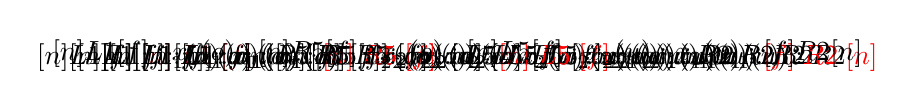
\begin{tikzpicture}
    \node<+> at(0,0){$\stackrel{\phantom\curvearrowright}{L1}:x_1(o):R5:x_2(o):L5:x_2(u):x_1(u):R2$};
    \node<+> at(0,0){${\color{red}\stackrel\curvearrowright{L1}}:x_1(o):R5:x_2(o):L5:x_2(u):x_1(u):R2$};
    \node<+> at(0,0){${\color{red}[n]\stackrel\curvearrowright{L1}[f]}:x_1(o):R5:x_2(o):L5:x_2(u):x_1(u):R2$};
    \node<+> at(0,0){$[n]\stackrel\curvearrowright{L1}[f]:x_1(o):{\color{red}\stackrel\curvearrowleft{R5}}:x_2(o):L5:x_2(u):x_1(u):R2$};
    \node<+> at(0,0){$[n]\stackrel\curvearrowright{L1}[f]:x_1(o):{\color{red}[n]\stackrel\curvearrowleft{R5}[f]}:x_2(o):L5:x_2(u):x_1(u):R2$};
    \node<+> at(0,0){$[n]L1[f]:x_1(o):[n]\stackrel\curvearrowleft{R5}[f]:x_2(o):{\color{red}\stackrel\curvearrowright{L5}}:x_2(u):x_1(u):R2$};
    \node<+> at(0,0){$[n]L1[f]:x_1(o):[n]\stackrel\curvearrowleft{R5}[f]:x_2(o):{\color{red}[n]\stackrel\curvearrowright{L5}[f]}:x_2(u):x_1(u):R2$};
    \node<+> at(0,0){$[n]L1[f]:x_1(o):[n]R5[f]:x_2(o):[n]\stackrel\curvearrowright{L5}[f]:x_2(u):x_1(u):{\color{red}\stackrel\curvearrowright{R2}}$};
    \node<+> at(0,0){$[n]L1[f]:x_1(o):[n]R5[f]:x_2(o):[n]\stackrel\curvearrowright{L5}[f]:x_2(u):x_1(u):{\color{red}[f]\stackrel\curvearrowright{R2}[n]}$};
    \node<+-> at(0,0){$[n]L1[f]:x_1(o):[n]R5[f]:x_2(o):[n]{L5}[f]:x_2(u):x_1(u):[f]{R2}[n]$};
\end{tikzpicture}
$$
\end{adjustwidth}

\only<4->{
\begin{center}
\begin{tabular}{c|c}
    \w{figures/leftcw.png}&\w{figures/rightcw.png}\\
    \hline
    \w{figures/leftccw.png}&\w{figures/rightccw.png}\\
\end{tabular}
\end{center}
}
% \only<12>{todo erase table, show string figure}
\end{frame}

\note[itemize]{
\item now that we can recover the string segments from the linear sequence
\item when we want to pick a specific string segment, we know where it is in the linear sequence
\item "use a finger to pick some segment" is essentially insert the finger to where the segment is in the linear sequence along with some crossings if needed

}